\documentclass[preprint,12pt,aps,pra,showkeys,amsmath,amssymb,superscriptaddress,floatfix]{revtex4-2}
\usepackage[T1]{fontenc}
\usepackage[utf8]{inputenc}
\usepackage{amsmath,amssymb,amsthm,mathtools,mathrsfs}
\usepackage{microtype,booktabs,enumitem}
\usepackage{xcolor,tikz,etoolbox}
\usepackage[skins,breakable]{tcolorbox}
\usepackage{needspace}
% Keep diagram geometry independent of REVTeX preprint body spacing.
\AtBeginEnvironment{tikzpicture}{\linespread{1}\selectfont}
\usetikzlibrary{arrows.meta,positioning,calc,fit,decorations.pathreplacing}
\usepackage{graphicx}
\usepackage{hyperref}

\definecolor{MMBlue}{RGB}{0,82,155}
\definecolor{MMOrange}{RGB}{200,80,0}
\tikzset{
 mmnode/.style={draw=MMBlue,rounded corners=2pt,fill=MMBlue!4,align=left,execute at begin node={\raggedright},text width=5cm,font=\fontsize{10}{12}\selectfont,inner sep=6pt},
 mmimport/.style={mmnode,draw=black!65,fill=black!4},
 mmcandidate/.style={mmnode,draw=MMOrange,dashed,fill=MMOrange!5},
 mmrejected/.style={mmnode,draw=black,densely dotted,fill=black!8},
 mmproof/.style={->,thick,MMBlue},
 mmflow/.style={->,semithick,black!70},
 mmrepair/.style={->,dashed,thick,MMOrange},
 mmcandidatearrow/.style={->,dashed,semithick,MMOrange},
 mmnote/.style={font=\scriptsize,fill=white,inner sep=2pt,align=center}}

\usepackage[section]{placeins}
\setlength{\emergencystretch}{3em}
\setlist{itemsep=3pt,topsep=4pt}
\newtheorem{theorem}{Theorem}[section]
\newtheorem{proposition}[theorem]{Proposition}
\newtheorem{lemma}[theorem]{Lemma}
\newtheorem{corollary}[theorem]{Corollary}
\theoremstyle{definition}
\newtheorem{definition}[theorem]{Definition}
\newtheorem{example}[theorem]{Example}
\theoremstyle{remark}
\newtheorem{remark}[theorem]{Remark}
% Avoid isolated statement headings and single-line paragraph fragments.
\BeforeBeginEnvironment{theorem}{\Needspace{6\baselineskip}}
\BeforeBeginEnvironment{definition}{\Needspace{5\baselineskip}}
\BeforeBeginEnvironment{proposition}{\Needspace{5\baselineskip}}
\BeforeBeginEnvironment{lemma}{\Needspace{5\baselineskip}}
\BeforeBeginEnvironment{corollary}{\Needspace{5\baselineskip}}
\clubpenalty=5000
\widowpenalty=5000
\newcommand{\R}{\mathbb R}\newcommand{\Z}{\mathbb Z}\newcommand{\N}{\mathbb N}
\newcommand{\Pa}{\operatorname{Pa}}\newcommand{\Desc}{\operatorname{Desc}}
\newcommand{\cl}{\operatorname{cl}}\newcommand{\cost}{\operatorname{cost}}
\newcommand{\status}{\operatorname{status}}
% Faculty cards: a visual rail groups the five faculties within one agent.
% The rail has no arrowhead and does not represent a proof dependency.
\newcommand{\mmfacultybadge}[1]{%
 \node[circle,draw=MMBlue,line width=1pt,fill=white,
 minimum size=7mm,inner sep=0pt,font=\sffamily\small\bfseries,text=MMBlue]
 at ([xshift=15pt,yshift=-15pt]frame.north west) {#1};}
\newcommand{\mmfacultyrail}{%
 \draw[MMBlue!80,line width=1pt]
 ([xshift=15pt,yshift=2pt]frame.north west)--
 ([xshift=15pt,yshift=-2pt]frame.south west);}
\newtcolorbox{mmfacultybox}[2]{enhanced,breakable,
 colback=MMBlue!4,colframe=MMBlue!4,boxrule=0pt,arc=3pt,
 left=39pt,right=9pt,top=4pt,bottom=4pt,
 before skip=2pt,after skip=2pt,
 fontupper=\small\linespread{1.1}\selectfont,
 overlay unbroken={\mmfacultyrail\mmfacultybadge{#1}},
 overlay first={\mmfacultyrail\mmfacultybadge{#1}},
 overlay middle={\mmfacultyrail},overlay last={\mmfacultyrail}}
\newcommand{\mmfaculty}[3]{%
 \begin{mmfacultybox}{#1}{#2}
 {\sffamily\bfseries\color{MMBlue}#2}\par\smallskip #3
 \end{mmfacultybox}}
\newcommand{\agent}[9]{%
 \Needspace{8\baselineskip}
 \subsubsection{#1}
 \noindent\textbf{Object.} #2\par
 \noindent\textbf{Role.} #3\par\smallskip
 \mmfaculty{E}{Ego}{#4}
 \mmfaculty{M}{Memory}{#5}
 \mmfaculty{I}{Intellect}{#6}
 \mmfaculty{S}{Sense}{#7}
 \mmfaculty{A}{Action}{#8}
 \smallskip\noindent #9\par}

\usepackage{longtable,array,calc}
\providecommand{\tightlist}{\setlength{\itemsep}{2pt}\setlength{\parskip}{0pt}}
\makeatletter
\def\frontmatter@abstract@produce{\par\addvspace{\frontmatter@preabstractspace}%
\begingroup\prep@absbox\unvbox\absbox\post@absbox\endgroup
\addvspace{\frontmatter@postabstractspace}}
\makeatother
\newcommand{\field}[2]{\par\smallskip\noindent\textbf{#1.} #2\par}
\setlength{\emergencystretch}{5em}
\AtBeginEnvironment{verbatim}{\small\linespread{1.0}\selectfont}


\hypersetup{colorlinks=true,linkcolor=MMBlue,urlcolor=MMBlue,pdfauthor={Dibakar Sigdel}}

\begin{document}

\title{Cantor's Theorem and the Power-Set Hierarchy\\[4pt]\large An End-to-End Meta-Math Walkthrough}

\author{Dibakar Sigdel}

\affiliation{Mindverse Computing LLC, Lynnwood, WA 98087, USA}

\date{October 2026}

\begin{abstract}

For any proposed enumeration of subsets, choose a new subset that
disagrees with the assigned subset at each element's own membership
test. The report presents the target theorem, declared imports, a
dependency graph, five-faculty node contracts, a continuous proof, a
worked example, and a hypothesis-repair audit. It is an authored
mathematical exposition, not a deployed-agent transcript or a formal
proof-assistant certificate.

\end{abstract}\maketitle\linespread{1.12}\selectfont

\noindent\textbf{LF-01 / Mathematical Logic and Set Theory / Report v1}

\section{Target and import contract}

\begin{theorem}

For every set \(A\), prove there is no surjection
\(f:A\to\mathcal P(A)\), where \(\mathcal P(A)\) is the set of all
subsets of \(A\). Since \(a\mapsto\{a\}\) is an injection, conclude that
\(A\) has strictly smaller cardinality than its power set, in the sense
of injection plus absence of a bijection. The diagonal argument does not
require the axiom of choice.

\end{theorem}

\subsection{Foundations and permitted imports}

Use the power-set and separation axioms of ordinary set theory, the
definitions of injective, surjective, and bijective functions, and
classical propositional logic. Separation permits forming a subset of an
already given set by a formula. No unrestricted ``set of all sets''
comprehension is used.

\clearpage\section{Node interaction workflow}

\begin{center}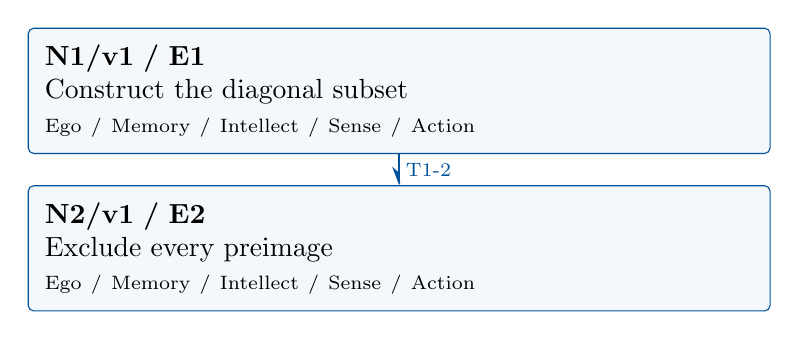
\begin{tikzpicture}[>=Stealth,x=1cm,y=1cm]

\node[mmnode,text width=9cm,minimum height=1.25cm] (N1) at (0,0.0) {\textbf{N1/v1 / E1}\\Construct the diagonal subset\\{\scriptsize Ego / Memory / Intellect / Sense / Action}};

\node[mmnode,text width=9cm,minimum height=1.25cm] (N2) at (0,-2.0) {\textbf{N2/v1 / E2}\\Exclude every preimage\\{\scriptsize Ego / Memory / Intellect / Sense / Action}};

\draw[mmproof] (N1.south) -- node[mmnote,right] {T1-2} (N2.north);

\end{tikzpicture}\end{center}

Each box is one mathematical agent containing all five faculties. Blue
arrows carry the versioned exports listed below. The layout gives a
reading order; only drawn arrows assert dependencies. Diagnostic repair
is separate from the proof DAG.

\subsection{Versioned evidence-transfer ledger}

\begingroup\small\linespread{1.05}\selectfont

\Needspace{5\baselineskip}\field{T1-2: N1/E1/v1 to N2}{\(D=\{a\in A:a\notin f(a)\}\) is a well-defined member of
\(\mathcal P(A)\).}

\field{Receiving activity}{N2.1}

\field{Compatibility}{E1/v1 and a hypothetical \(b\in A\) with \(f(b)=D\). Check: The
contradiction applies to every proposed surjection, including finite and
empty domains.}

\endgroup

\clearpage\section{Agent roles and five-faculty activities}\begingroup\small\linespread{1.05}\selectfont\setlist{itemsep=1pt,topsep=2pt}

\subsection{N1/v1: Construct the diagonal subset}

\field{Object and role}{Use bounded separation to reverse each element's own membership
decision. \textbf{Local obligation:} \(D=\{a\in A:a\notin f(a)\}\) is a
well-defined member of \(\mathcal P(A)\).}

\field{Inputs}{An arbitrary function \(f:A\to\mathcal P(A)\).}

\mmfaculty{E}{Ego}{Publish E1/v1 only after establishing this obligation:
\(D=\{a\in A:a\notin f(a)\}\) is a well-defined member of
\(\mathcal P(A)\).}

\mmfaculty{M}{Memory}{An arbitrary function \(f:A\to\mathcal P(A)\). Retain the stated
assumptions and import versions.}

\mmfaculty{I}{Intellect}{Use bounded separation to reverse each element's own membership
decision.}

\mmfaculty{S}{Sense}{The definition produces a subset of \(A\), so it belongs to the
codomain; no self-containing universal set is needed.}

\mmfaculty{A}{Action}{Carry out activities N1.1--N1.2 below, retaining each calculation and
construction as evidence.}

\smallskip\noindent\textbf{Numbered mathematical activities}

\begin{enumerate}[label=N1.\arabic*,leftmargin=3.4em]

\item For each \(a\in A\), \(f(a)\) is a subset of \(A\), so the membership
statement \(a\in f(a)\) is meaningful. By separation, the elements of
\(A\) for which this statement is false form a set \(D\subset A\).

\item The definition gives, for each \(a\in A\), the exact equivalence
\(a\in D\iff a\notin f(a)\). In particular \(D\) is in the stated
codomain \(\mathcal P(A)\).

\end{enumerate}

\field{Export E1/v1}{\(D=\{a\in A:a\notin f(a)\}\) is a well-defined member of
\(\mathcal P(A)\).}

\field{Acceptance gate}{The definition produces a subset of \(A\), so it belongs to the
codomain; no self-containing universal set is needed.}

\field{Targeted repair}{If the construction is made over all sets rather than \(A\), restrict it
to \(A\); bounded separation is the actual permitted axiom. Withhold
this export and recheck its descendants after a versioned correction.}

\clearpage

\subsection{N2/v1: Exclude every preimage}

\field{Object and role}{Specialize the membership equivalence at the alleged preimage and derive
a contradiction. \textbf{Local obligation:} No \(f:A\to\mathcal P(A)\)
is surjective; the singleton map establishes strict cardinal growth.}

\field{Inputs}{E1/v1 and a hypothetical \(b\in A\) with \(f(b)=D\). Incoming proof
exports: E1/v1 at N2.1.}

\mmfaculty{E}{Ego}{Publish E2/v1 only after establishing this obligation: No
\(f:A\to\mathcal P(A)\) is surjective; the singleton map establishes
strict cardinal growth.}

\mmfaculty{M}{Memory}{E1/v1 and a hypothetical \(b\in A\) with \(f(b)=D\). Incoming proof
exports: E1/v1 at N2.1. Retain the stated assumptions and import
versions.}

\mmfaculty{I}{Intellect}{Specialize the membership equivalence at the alleged preimage and derive
a contradiction.}

\mmfaculty{S}{Sense}{The contradiction applies to every proposed surjection, including finite
and empty domains.}

\mmfaculty{A}{Action}{Carry out activities N2.1--N2.2 below, retaining each calculation and
construction as evidence.}

\smallskip\noindent\textbf{Numbered mathematical activities}

\begin{enumerate}[label=N2.\arabic*,leftmargin=3.4em]

\item If \(f(b)=D\), the equivalence in E1 reads \(b\in D\iff b\notin D\),
impossible in classical logic. Thus no element of \(A\) maps to \(D\),
and the arbitrary function \(f\) is not surjective.

\item The singleton map \(a\mapsto\{a\}\) is injective because equal singleton
sets have equal elements. A bijection would in particular be a
surjection, already ruled out. This proves the claimed strict cardinal
comparison. For \(A=\varnothing\), \(\mathcal P(A)=\{\varnothing\}\) and
the same lack of surjection is immediate.

\end{enumerate}

\field{Export E2/v1}{No \(f:A\to\mathcal P(A)\) is surjective; the singleton map establishes
strict cardinal growth.}

\field{Acceptance gate}{The contradiction applies to every proposed surjection, including finite
and empty domains.}

\field{Targeted repair}{If a contradiction is interpreted as showing the power set is
inconsistent, identify the rejected assumption: only the proposed
surjectivity fails. Withhold this export and recheck its descendants
after a versioned correction.}

\endgroup\clearpage\section{Continuous mathematical proof}\label{sec:proof}

\subsection{N1 --- Construct the diagonal
subset}\label{n1-construct-the-diagonal-subset}

\begin{enumerate}
\def\labelenumi{\arabic{enumi}.}
\item
  \textbf{N1.1.} For each \(a\in A\), \(f(a)\) is a subset of \(A\), so
  the membership statement \(a\in f(a)\) is meaningful. By separation,
  the elements of \(A\) for which this statement is false form a set
  \(D\subset A\).
\item
  \textbf{N1.2.} The definition gives, for each \(a\in A\), the exact
  equivalence \(a\in D\iff a\notin f(a)\). In particular \(D\) is in the
  stated codomain \(\mathcal P(A)\).
\end{enumerate}

\subsection{N2 --- Exclude every
preimage}\label{n2-exclude-every-preimage}

\begin{enumerate}
\def\labelenumi{\arabic{enumi}.}
\item
  \textbf{N2.1.} If \(f(b)=D\), the equivalence in E1 reads
  \(b\in D\iff b\notin D\), impossible in classical logic. Thus no
  element of \(A\) maps to \(D\), and the arbitrary function \(f\) is
  not surjective.
\item
  \textbf{N2.2.} The singleton map \(a\mapsto\{a\}\) is injective
  because equal singleton sets have equal elements. A bijection would in
  particular be a surjection, already ruled out. This proves the claimed
  strict cardinal comparison. For \(A=\varnothing\),
  \(\mathcal P(A)=\{\varnothing\}\) and the same lack of surjection is
  immediate.
\end{enumerate}

\hfill$\square$

\section{Worked orchestration}

For \(A=\{1,2,3\}\), consider \(f(1)=\{1,2\}\), \(f(2)=\{1\}\), and
\(f(3)=\{3\}\). The diagonal rule includes \(2\) but excludes \(1\) and
\(3\), so \(D=\{2\}\). It is different from all three listed images,
illustrating the exact self-index disagreement.

\subsection{Boundary and hypothesis audit}

Listing all finite subsets of \(\mathbb N\) is possible and does not
contradict Cantor: the codomain is then only a proper part of
\(\mathcal P(\mathbb N)\). The diagonal subset for such a list cannot be
one of its listed finite subsets. Replacing ``all subsets'' by ``finite
subsets'' changes the target.

\section{Illustrative failure and repair}

The following is an authored diagnostic scenario. Changed assumptions
define a new contract; they do not retroactively prove the original
statement.

\subsection{Rejected argument, diagnosis, and correction}
\textbf{Rejected scope (N1):} form the set of all sets that do not
contain themselves. \textbf{Diagnosis:} Memory replaced separation over
\(A\) by unrestricted comprehension. \textbf{Repair:} construct only
\(D\subset A\) using the given map; its existence is licensed by
separation. Then N2 contradicts surjectivity, not the set axioms.
Recheck the codomain membership and final cardinal comparison.

\subsection{Publication and reuse}
The corrected export retains its explicit assumptions. A hypothetical
revision receives a new version, and each consuming activity is
rechecked; this scenario is not a recorded runtime event. \textbf{Next
direction:} Apply the construction to \(A=\mathbb N\) to obtain an
uncountable power set and to explain why no single list can enumerate
all binary sequences.

\par\medskip\begingroup\small\linespread{1.0}\selectfont\noindent\textbf{Provenance.} This authored proof is complete relative to its declared imports. Reuse
each export with its assumptions, proof, and version. The original
Markdown remains available for comparison.
\par\endgroup

\par\smallskip\begingroup\small\linespread{1.0}\selectfont\noindent\textbf{Further reading.} \href{https://math.berkeley.edu/~marks/notes/set_theory_notes_4.pdf}{Andrew
Marks, Set Theory notes} for sets and ultraproducts;
\href{https://math.berkeley.edu/~antonio/math125A/mathlogicP1.pdf}{Berkeley,
Mathematical Logic for Mathematicians, Part I} for first-order
semantics;
\href{https://math.berkeley.edu/~marks/notes/computability_notes_v1.pdf}{Andrew
Marks, Computability Theory notes} for effective procedures and
undecidability. The proofs below specify their own set-theoretic and
semantic assumptions.\par\endgroup

\end{document}
